%%%%%%%%%%%%%%%%%%%%%%%%%%%%%%%%%%%%%%%%%%%%%%%%%%%%%%%%%%%%%%%%%%%%%%%%%%%%%%%%%%%%%%%%%%%%%%%%%%%%
\documentclass[11pt,letterpaper]{article}
\usepackage[applemac]{inputenc}
\usepackage[centertags]{amsmath}
\usepackage{amsthm}
\usepackage{amssymb}
\usepackage{mathrsfs}
\usepackage{graphicx}
\usepackage{amsfonts}
%\usepackage{authblk}
%\usepackage{pstricks, pst-plot}
%\usepackage{tikz}
%\usetikzlibrary{calc,shapes,positioning,shadows,arrows}
\usepackage{color}
\usepackage{xcolor}
\usepackage{multirow}
\usepackage{natbib}
%\pagestyle{headings}
\usepackage{hyperref}

\usepackage{colortbl}
\usepackage{comment}

%\decimalpoint

\usepackage{fancyhdr}
\parindent 1cm
\parskip 0.2cm
\topmargin -1cm
\oddsidemargin 0cm
\evensidemargin 0cm
\textwidth 16.5cm
\textheight 22cm

\setlength\parindent{0pt}
\setlength{\parskip}{1em}


\title{
{\textbf{\large{Australian and New Zealand Statistical Journal}}} \vspace{1cm}\\ 
A Bayesian generalized additive mixed model under monotone constraints 
\vspace{1cm}\\

}

%%% en aplicaciones biom\'edicas

\author{
Lizbeth Naranjo Albarr\'an$^{1}$, V\'ictor Miranda Soberanis$^{2}$,  Patricio Maturana Russel$^{2}$   
}

\date{
$^{1}$Departamento de Matem\'aticas, Facultad de Ciencias, Universidad Nacional Aut\'onoma de M\'exico, Mexico City, Mexico.  \\
$^2$ Department of Mathematical Sciences, Auckland University of Technology, Auckland, New Zealand.  
}

\begin{document}

\maketitle

\begin{abstract}
A Bayesian approach  is proposed to consider continuous response subject to monotone constraints.  A generalized additive model with fixed and random effects has been introduced to consider the monotonic process via constraints on the smoothing functions, either decreasing or increasing patterns. Some particular data exemplify the proposal, for which the monotony on the longitudinal  response variable is addressed by the monotony on the smoothing function of an explanatory variable.   
\end{abstract}

\textbf{Keywords:} 
Bayesian statistics; 
Generalized additive models; 
Integrated penalized splines; 
Longitudinal data; 
Monotone constraints; 
Random effects. 


\section{Introduction}\label{sec:intro}


%\textbf{*Parag. La necesidad de extender los GLM y trabajar con modelos aditivos GAM*}  \\  

Generalized additive models (GAM) \citep{HasTib90, Woo17, Yee15} are a non-parametric extension of generalized linear models (GLM), to study the relationship between a response variable and a set of explanatory variables. 
The GLM were proposed by \cite{NelWed72}, and are an extension of the linear model, to be able to include models for data with binary and count responses, among others.   
The GAM arises from the need to extend the linear relationships  in the GLM, in order to include non-linear relationships. 
Several R packages have been implemented with the need to use  GAM, for instances \texttt{VGAM} \citep{Yee10}, \texttt{VGAMextra} \citep{VGAMextra}, and \texttt{mgcv} \citep{Woo17,Woo16}.  
To include these non-linear relationships in GAM, non-parametric smoothing functions are used, such as  nearest-neighbour smoothers, regression or series smoothers, local regression or smoothing splines. 


% \textbf{*Parag. GLM con restricciones crecientes/decrecientes*} \\ 

Statistical modeling depends on accurate data to obtain reliable results. 
In the model parameter estimation process,  sometimes it is necessary to include constraints on the parameters so that the estimation process is possible, or to have the necessary characteristics required by the data. 
For instance, the well known constraints studied by \cite{GouHolMon82}, where they considered the problem of testing statistical hypotheses in linear regression models with inequality constraints on the regression coefficients.    
It is such that monotony scenarios can be considered as particular cases, which in the case of GLM are translated into constraints such that the parameters are positive or negative.


%\textbf{*Parag. Splines con restricciones crecientes/decrecientes*} \\ 
 
For the GAM many of the works developed on smoothing functions are based on splines, due to their ease of handling and estimation process. 
In addition, various proposals on splines have arisen to address constraints such that the monotony. 
Monotone regression spline estimators were defined by \cite{Ram88}.  
Another project was developed by Mary C. Meyer, where she proposed  algorithms for the cubic monotone and  convex constraints,  and variants such as increasing-concave \citep{Mey08,Mey12}. 
\cite{ShiWalDam11} used free-knot and fixed-knot regression splines to develop methods for the nonparametric estimation of functions subject to shape constraints in models with log-concave likelihood functions in a Bayesian context; they considered monotonicity, convexity and functions with a single minimum.  


% \textbf{*Parag. Otros trabajos de GAM con restricciones crecientes*} \\

In GAM some proposals have been developed to extend some restrictions such as monotonicity. 
\cite{BreSte08} proposed a Bayesian approach for monotonic regression using penalized B-splines.  
\cite{CaiLinWan11} proposed a Bayesian approach to model the baseline cumulative hazard function with monotone splines leading to only a finite number of parameters to estimate while maintaining great modeling flexibility. 
 \cite{PyaWoo15} developed GAM under shape constraints on the components functions by using the SCOP-splibes, and they implemented the proposal on the \texttt{R} package \texttt{scam}.  
The work on splines of Mary C. Meyer has been extended to GAM with shape and order restrictions \cite{Mey18}, and implemented in \texttt{R} package  \texttt{cgam} \cite{LiaMey19},  where they addressed monotonicity, convexity, their combinations, tree, umbrella orderings, by suing Gaussian, Poisson, and binomial distribution for the response variable.    
Recently, \cite{SpiKneOtt19} present eda flexible approach based on maximum likelihood estimation, for response function estimation using monotonic P-splines with additive predictors as in GAM. 


%\textbf{*Parag. Propuesta del articulo*}  

The approach begins a generalized additive  model, where some of the additive terms are constrained to be monotonic. The additive proposal is based on monotonic functions by using penalized integrated basis functions, known as  penalized I-splines,  having either decreasing or increasing patterns.   Then, it is extended to address the monotonic constraint in a repeated measured structure for longitudinal datasets. 
Our proposed approach has been motivated by and applied to three longitudinal studies, for which the disease nature should have monotone patterns. 


% \textbf{*Parag. Outline*} 

The outline of this paper is as follows. 
In section \ref{sec:motiva} motivation data are described to motive the proposal. 
In section \ref{sec:review} a review on GAM and splines is given. 
Section \ref{sec:approach} the proposed model is defined. 
The Bayesian analysis is obtained in Section  \ref{sec:bayes}.
The applications of the proposal is presented in section \ref{sec:examples}. 
Finally, the conclusions are discussed in section \ref{sec:conclusion}. 


%\textbf{*Parag. Sobre las ventajas del metodo Bayesiano*} \\ 
%Bayesian approach allows the advantages that constraints are taken into account in the prior distribution, and consequently in the posterior distribution. 



\section{Motivating problems}\label{sec:motiva}

In this section we introduce some data that motivate the development of this article and that will exemplify the proposed approach.



\subsection{Aortic aneurysm progression data}  


The dataset \texttt{aneur}, available in the R package \texttt{msm} \cite{Jac11}, contains longitudinal measurements of grades of aortic aneurysms, they are measured by ultrasound examination of the aorta diameter. 

The data correspond to ultrasound scans from 838 men over 65 years of age. 
The data frame contains the following variables: 
\texttt{ptnum}= patient identification number; 
\texttt{age}= recipient age at examination (years); 
\texttt{diam}= aortic diameter (mm); 
\texttt{state}= stage of aneurysm. 
The \texttt{state} variable is defined from the \texttt{diam} by categorizing in an ordinal scale: 
\texttt{state 1}= aneurysm-free (diam $<$ 30 mm), 
\texttt{state 2}= mild aneurysm (diam 30-44 mm), 
\texttt{state 3}= moderate aneurysm	(diam 45-54 mm), 
\texttt{state 4}= severe aneurysm (diam $>$ 55 mm). 
The data used in this paper is  a subset of 229 men whose aortic diameters presented at least one different value along time. 



The disease has a degenerative nature, therefore aortic diameter is expected to remain in the same condition or grow over time, i.e. they should be non-decreasing over age. However, in Figure \ref{fig:aneur.1data} data displays different patterns, some of which do not comply with the non-decreasing monotonicity constraint. Therefore, monotonic constraints could help to model the disease degenerative nature. 

 \begin{figure}[!htb]
\centering
\begin{tabular}{@{\hspace{0mm}}c@{\hspace{1mm}}c@{\hspace{0mm}}}
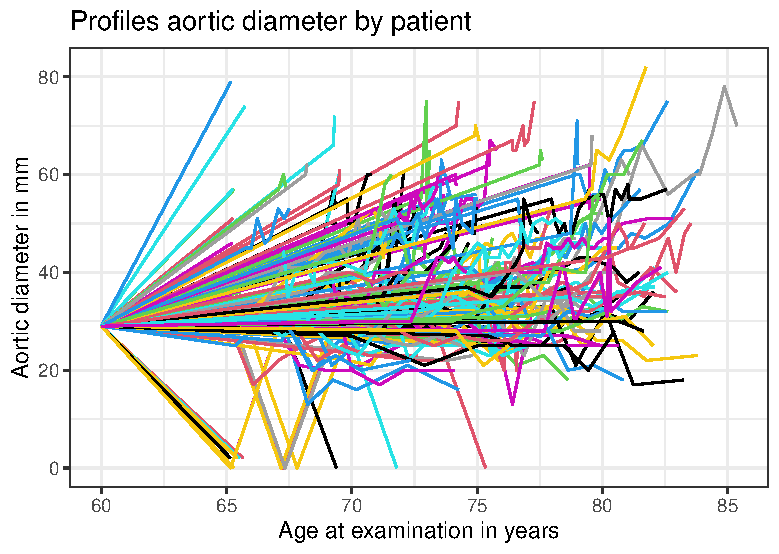
\includegraphics[scale=0.6]{Figures/fig_aneur_1diam} &
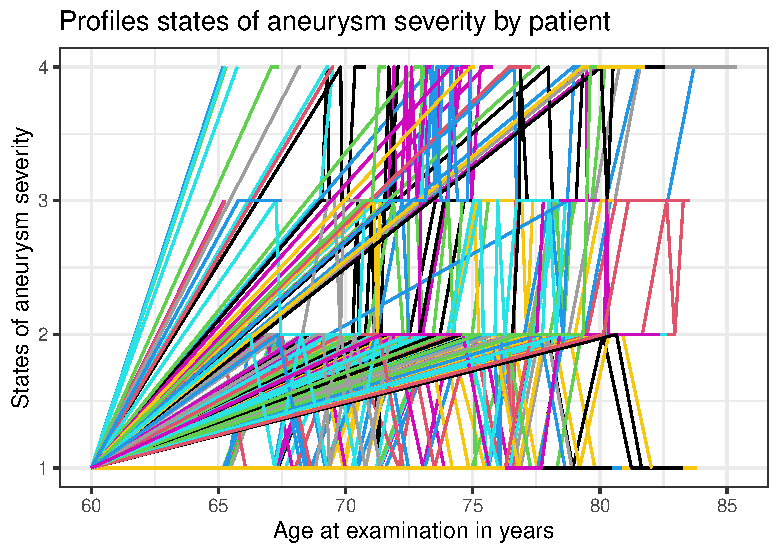
\includegraphics[scale=0.6]{Figures/fig_aneur_1state} 
\end{tabular}
%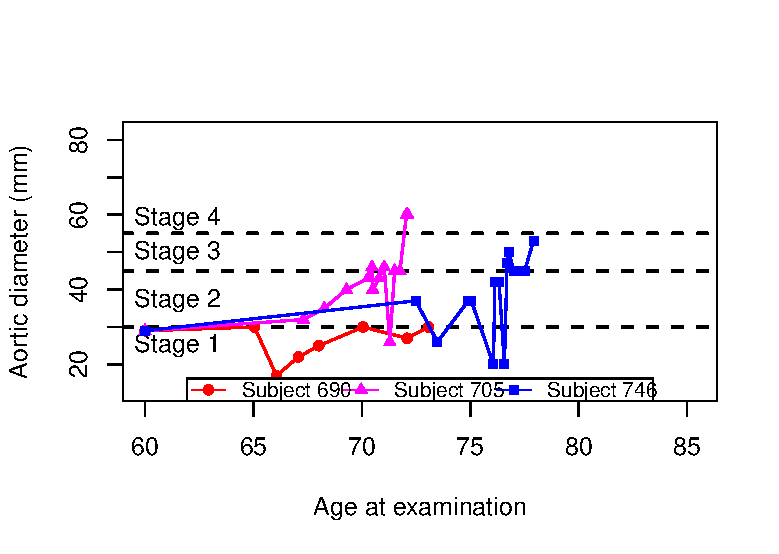
\includegraphics[scale=0.6]{Figures/fig_aneur_1cases} 
\caption{Aortic aneurysm progression data.}\label{fig:aneur.1data}
\end{figure}



\subsection{UPDRS scores data}

\cite{Tsa10} used the information and voice recordings of 42 out of 52 patients  having idiopathic Parkinson disease (PD) diagnosed, who remained in the trial of the AHTD study presented by \cite{Goetz09}. The  features  extracted from the voice recordings  of these 42 patients (28 men and
14 women) were analyzed by \cite{Tsa10}, and are available online at the UCI Machine Learning Repository
(\url{https://archive.ics.uci.edu/ml/datasets/Parkinsons+Telemonitoring}). 
Patients could not be on symptomatic therapies for PD. Inclusion criteria considered that the patients could remain untreated during the study period of 6 months. 
The subjects were physically assessed and assigned Unified Parkinson's Disease Rating Scale (UPDRS) scores at baseline, 3 months, and 6 months later into the trial. During the trial  six phonations of sustained /a/ were recorded weekly for each patient.  

The database contains the age, gender, time interval from baseline recruitment date, motor UPDRS and total UPDRS (the real for baseline, three and six months, and the interpolated values around weekly),  and 16 biomedical voice measures. 
For this paper we have used only six features:  
Jitter in Percentage (JittP), 
Local Shimmer (LShimm), 
Harmonic-to-Noise Ratio (HNR), 
Recurrence Period Density Entropy (RPDE), 
Detrended Fluctuation Analysis (DFA), and
Pitch Period Entropy (PPE).


Due to patients  were not treated, and due to PD is a progressive disease for which  symptoms do not improve without medication,  it is expected that UPDRS scores are non-decreasing. However,  Figure \ref{fig:updrs.1data} displays the data showing some of the measures do not have non-decreasing patterns. Therefore, monotonic constraints would help to model the disease progression. 


\begin{figure}[!htb]
\centering
\begin{tabular}{@{\hspace{0mm}}c@{\hspace{1mm}}c@{\hspace{1mm}}c@{\hspace{0mm}}}
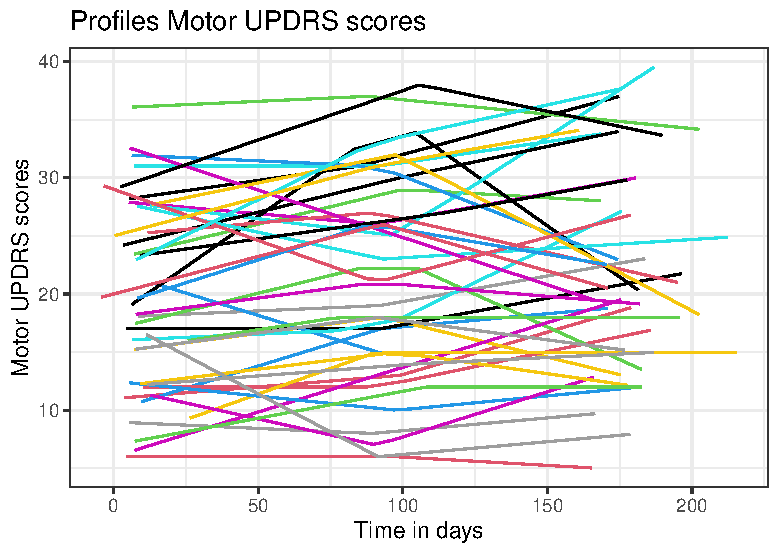
\includegraphics[scale=0.6]{Figures/fig_updrs_1motor} &
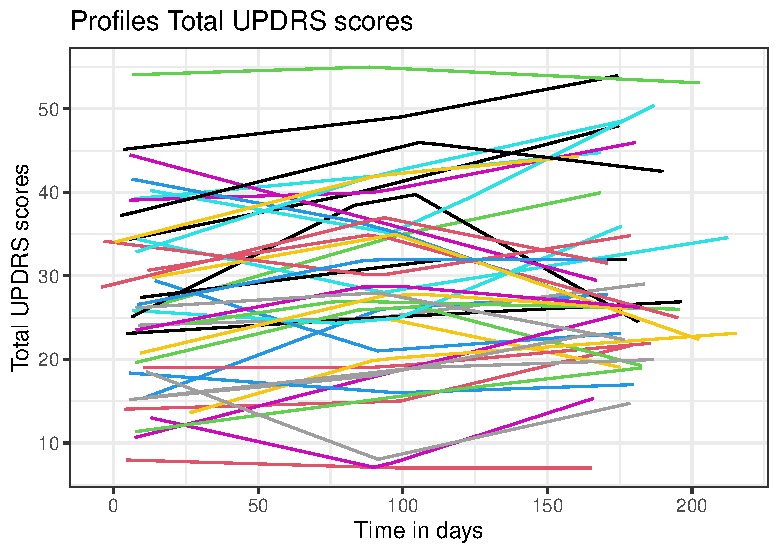
\includegraphics[scale=0.6]{Figures/fig_updrs_1total} 
\end{tabular}
\caption{Profiles of the UPDRS scores data.}\label{fig:updrs.1data}
\end{figure}






\subsection{HIV: CD4-CD8 ratio and Adherence}


%%%****FALTA Pedir las datos prestados a Doctores de Nutricion**** \\


The HIV infection progression is characterized by a progressive decrease of CD4+T lymphocytes  counts and an increase of CD8+T lymphocytes  counts, and therefore a simultaneous decrease of CD4/CD8 ratio.
The HIV viral load and CD4+T lymphocytes counts are the biomarkers most used to monitor HIV-positive patients, and also the CD4/CD8 ratio has been used as a biomarker.  
In addition, antiretroviral adherence in people with HIV and virological suppression has associated with a decreased CD4-CD8 ratio.

Usually, those relationships found are based on statistical models with linear relationships. However,   if we look for a more flexible non-linear relationship between ART adherence and CD4-CD8 ratio, it may result in a pattern that does not necessarily show the nature of the data, as it is displayed in the  Figure \ref{fig:hiv.1data}, where data have a valley for male at about ART adherence 98-100 and a peak for female at about ART adherence 94-100, most probably due to the lack of information or to the nature of data collection.   Therefore, monotonic constraints would help to model the natural patterns avoiding peaks and valleys in the fit. 


\begin{figure}[!htb]
\centering
\begin{tabular}{@{\hspace{0mm}}c@{\hspace{1mm}}c@{\hspace{0mm}}}
%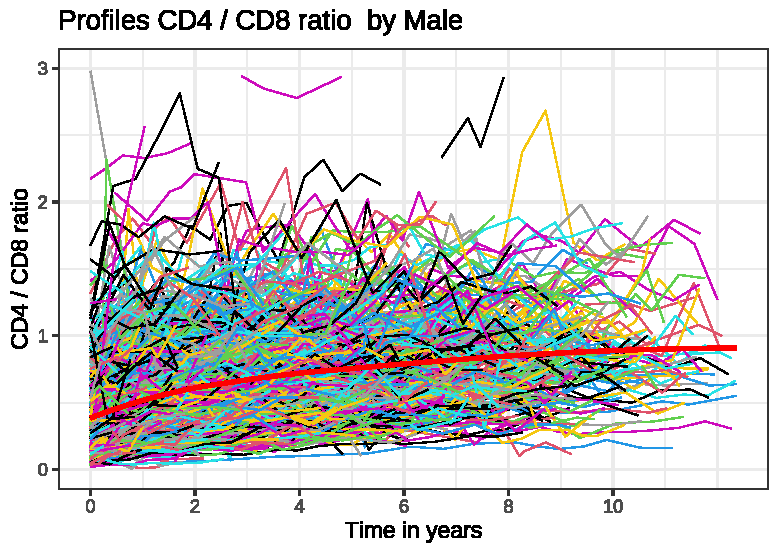
\includegraphics[scale=0.6]{Figures/fig_hiv1_cd4cd8_time_male} &
%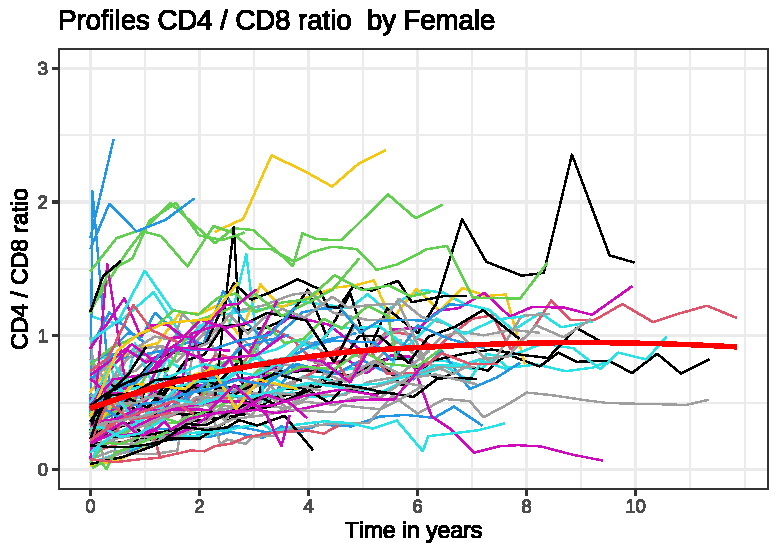
\includegraphics[scale=0.6]{Figures/fig_hiv1_cd4cd8_time_female}  \\
%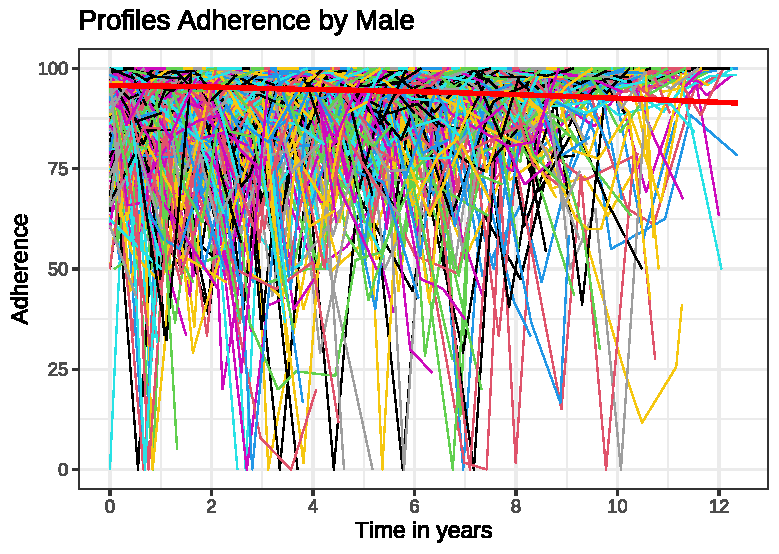
\includegraphics[scale=0.6]{Figures/fig_hiv1_adh_time_male} &
%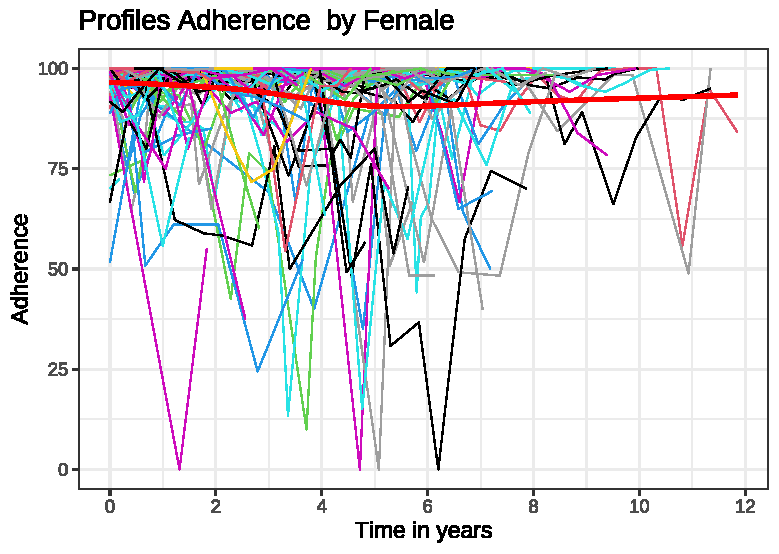
\includegraphics[scale=0.6]{Figures/fig_hiv1_adh_time_female}  \\
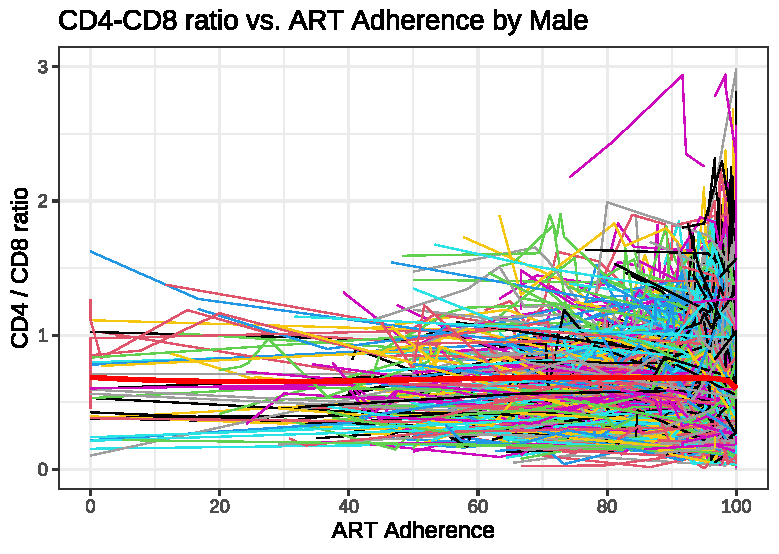
\includegraphics[scale=0.6]{Figures/fig_hiv1_cd4cd8_adh_male} &
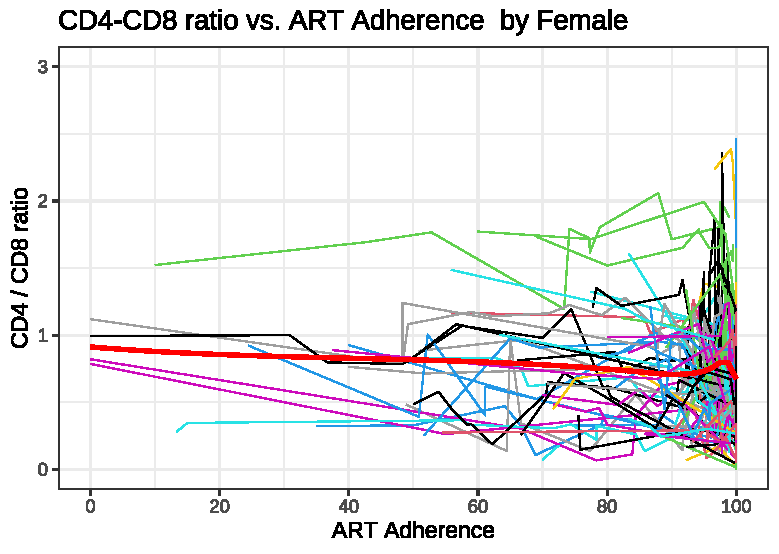
\includegraphics[scale=0.6]{Figures/fig_hiv1_cd4cd8_adh_female} 
\end{tabular}
\caption{Profiles of CD4-CD8 ratio by ART adherence. Footnote: fat red line represents average pattern. }\label{fig:hiv.1data}
\end{figure}



%\subsection{OTROS Posibles datos} 
%\begin{itemize} 
%\item Ejemplos del paquete cgam: Rubber, o plasma retinol. 
%\item Datos conocidos de diabetes Pima Indian Women 
%\end{itemize} 




\section{A review} \label{sec:review} 
 
In this section we give a brief review about GAM, the smoothing functions by using B-splines and P-splines, and  GAM for fixed and random effects. 
 
 \subsection{Generalized additive models}
 
% \paragraph{Introducir los GAM}
Suppose we have the response variable $Y$, defined as a random variable with a distribution belonging to the exponential familiy,  
\begin{eqnarray*}
p(y;\theta,\phi) &=& \exp\left[\left\{y\theta-b(\theta)\right\}/a(\phi)-c(y,\phi)\right], 
\label{eq:exponential.family}
\end{eqnarray*}
where $\theta$ is the canonical parameter, $\phi$ is the known dispersion parameter,  and $a(\phi)$, $b(\theta)$, and  $c(y,\phi)$ are functions of $\phi$,  $\theta$, and  $y$ and $\phi$, respectively.  
The link function $g(\cdot)$ is defined to relate the mean  $\mu=\mathbb{E}(Y)$ and the linear predictor $\eta$, as $g(\mu)=\eta$. The required properties for $g(\cdot)$ are such that it must be strictly monotonic and twice differentiable in the range of $\mu$; and its main purpose is to transform the mean, and often helps with interpretability.  
In the case of generalized linear models (GLM)  \citep{NelWed72} the linear predictor $\eta$ is a linear combination of the predictor variables  $\boldsymbol{x}=(x_1,x_2,\ldots,x_p )$, that is, $\eta = x_{1}\beta_1 + \cdots + x_{p}\beta_p = \boldsymbol{X}\boldsymbol{\beta}$. In the case of generalized additive models (GAM) \citep{HasTib90} the effects of the covariates are assumed to be additive, therefore in order to allow flexible non-linear curves, it is necessary that  
the systematic component $\eta$ is defined as a sum of smooth functions of the explanatory variables: 
\begin{eqnarray*}
g(\mu(\boldsymbol{x}))&=&\eta \quad=\quad f_1 (x_1 )+f_2 (x_2 )+\cdots+f_p (x_p ) , 
\end{eqnarray*}
where $f_1,\ldots,f_p$  are non-parametric smoothing functions, that allow modeling the non-linear effect that some covariates may have. And also, as a particular case it is possible to consider linear relationships using $f_k(x_k)=x_k\beta_k$, $k=1,\ldots,p$. 
Usually, the intercept is included as $f_1 (x_1 )=\beta_0$, and the $f_k$'s are centered for identifiability purposes. 

%\paragraph{Smoothing methods}  
The smoothing functions $f_k$ allow the linear relationship to be extended to other sophisticated non-linear effects. 
In GAM different smoothing functions can be used to estimate $f_k$,  four broad categories of smoothers are:   
regression or series smoothers,  smoothing splines,  local regression, and nearest-neighbour smoothers.    
Details are described in  \cite{JamWitHasTib13}, \cite{Yee15}, and \cite{Woo17}. In this paper we will use the penalized spline  basis functions, also known as P-splines or penalized B-splines.


\subsection{B-splines and P-splines \label{sec:b.p.splines}}

A \textit{spline} is a function defined piecewise by polynomials. For a spline of order $Q$, each piece is defined usually by  low degree polynomials, of order $\leq Q-1$ (usually degree 3 or lower), on a $x$-region that is delimited by \textit{knots} (breakpoints). The $(x,y)$ positions where each pair of segments join are called \textit{joints}. The piecewise polynomials are forced to join smoothly at the knots, and to guarantee this smoothness usually it is required having continuous zeroth, first and second derivatives. The most popular are the cubic splines, defined as  piecewise cubic polynomials ($Q-1=3$), i.e. splines of order $Q=4$.  



The \textit{B-splines} of order $Q$ are basis functions for spline functions defined over the same knots, both having the same order.  
This means that any spline function can be expressed by a linear combination of B-splines;  and for each spline function there is only one unique combination. 
Suppose that $x\in[a,b]$, usually normalizing $x\in[0,1]$, and let define the smoothing function:  
\begin{eqnarray}
f(x) &=& 
\sum_{s=1}^{K+Q} B_{s,q}(x) \beta_{s},   
\label{eq:basis.function}
\end{eqnarray} 
where  $\beta_{s}$ are unknown parameters,  and $B_{s,q}(x)$ denotes the $s$th B-spline basis function of order $q$ (degree $q-1$), for the knot sequence $\boldsymbol{\xi}$ for $q=1,\ldots,Q$.  There are many possibilities to define the basis function, for instance the ones given in \cite{Yee15} are described below. 

Assume there are $K$  interior knots $\xi_s$, $s=1,\ldots,K$, which are fixed knots either equidistant or equiprobable, and let $\xi_0$ and $\xi_{K+1}$ be the two boundary knots. 
These knots are augmented with $2Q$ others  to obtain a vector $\boldsymbol{\tau}=(\tau_1,\ldots,\tau_{K+2Q})$, such that,  
\begin{eqnarray*} 
\tau_1\leq\cdots\leq\tau_{Q} \ \leq \ \xi_{0} \ < \
 \xi_{1}\leq\cdots\leq\xi_{K}  
 \ < \ \xi_{K+1}\ \leq \ \tau_{K+Q+1}\leq\cdots\leq\xi_{K+2Q} , 
\end{eqnarray*} 
where $\tau_{Q+s}=\xi_s$ for $s=1,\ldots,K.$ Usually   $\tau_1=\cdots=\tau_Q=\xi_0$ and $\tau_{K+Q+1}=\cdots=\tau_{K+2Q}=\xi_{K+1}$.  
Then, the B-spline basis function are defined recursively as:
\begin{eqnarray*}
B_{s,1}(x) &=& \begin{cases}
1 & \xi_{s}\leq x<\xi_{s+1} , \\ 
0 & \text{otherwise}, \\
\end{cases}
\\
B_{s,q}(x) &=& w_{s,q}B_{s,q-1}(x) + (1-w_{s+1,q}) B_{s+1,q-1}(x) , 
\end{eqnarray*}
for $s=1,\ldots,K+2Q-q$ and $q>1$, 
where 
$w_{s,q} = 
({x-\xi_{s}})/({\xi_{s+q-1}-\xi_{s}})$  if $\xi_{s+q-1}>\xi_{s}$, and   
$w_{s,q}=0$ if $\xi_{s+q-1}=\xi_{s}$.  

 





%\paragraph{P-splines} 
The \textit{P-splines}, or penalized B-splines,   are extensions of the regression splines where the coefficients of adjacent B-splines are penalized. 
The  B-splines  depend on the number of knots $K$ and the positioning of the basis functions  $B_{s,q}(x)$; the number of knots $K$ is chosen to be large enough to avoid  over-smoothing, but small enough to avoid excessive computational cost.  However,  the P-splines avoid that dependency by considering a large number of basis functions subject to the smoothness condition that the coefficients of the neighboring basis functions must not differ too much.


The flexibility of $f$ is  controlled in less part by $K$, and in large part by the imposition, during fitting, of a quadratic smoothing penalty of the form:  
\begin{eqnarray*} 
\lambda \boldsymbol{\beta}^{T} \boldsymbol{P} \boldsymbol{\beta}  , 
\end{eqnarray*} 
where $\lambda>0$ is the smoothing parameter that must be estimated, and the $\boldsymbol{P}$ is a matrix of known coefficients. 
The penalty matrix es defined as $\boldsymbol{P}=\boldsymbol{D}^{T}\boldsymbol{D}+\varepsilon\boldsymbol{I}_{K-1}$ (which s a full rank matrix for any small quantity $\varepsilon$, for instance, $10^{-6}$), and $\boldsymbol{D}$ is the $d$th order difference matrix ($d=1,2,\ldots,K-2$) of dimension $(K-1-d)\times(K-1)$. In practice, a common value is $d=2$, its operator of differentiation  is  $\Delta^2\beta_s = \Delta(\Delta\beta_s) = \Delta\beta_s-\Delta\beta_{s-1} = \beta_s-\beta_{s-1}-(\beta_{s-1}-\beta_{s-2})  =  \beta_s- 2\beta_{s-1}+\beta_{s-2}$, and  the difference matrix is: 
\begin{eqnarray*}
\boldsymbol{D}_{[2]} &=& 
\left[\begin{array}{cccccccccc} 
1&-2&1&0&0&\cdots&&&&0 \\
0&1&-2&1&0&\cdots&&&&0 \\
\vdots&&\ddots&\ddots&\ddots&&\ddots&\ddots&\ddots& \\
0&0&&&&\cdots&0&1&-2&1 \\
\end{array}\right]_{(K-3)\times(K-1)} .
\end{eqnarray*}



%Note that $f(x)$ can be written as $f=\boldsymbol{X}\boldsymbol{\beta}$ where the element $(i,j)$ of matrix $\boldsymbol{X}$ is $\boldsymbol{X}[{i,j}]=B_{j,Q}(x_{i})$. 


To see the smoothers with Bayesian methods, the penalties can be induced by means of multivariate Gaussian improper prior distributions, having precision matrices proportional to $\sum_{j} \lambda_j \boldsymbol{P}_j$. See more details in \cite{LanBre04}. 


\subsection{Generalized additive mixed models} 

Mixed models are an extension of simple models to allow both fixed and random effects, and they are used when data are not independent, as in hierarchical,  longitudinal, or correlated structures. 
A linear mixed model (LMM) is defined as:  
\begin{eqnarray*}
\boldsymbol{y}_i &=& \boldsymbol{X}_i\boldsymbol{\beta} + \boldsymbol{Z}_i\boldsymbol{b}_i + \boldsymbol{\varepsilon}_i, 
\qquad 
\boldsymbol{b}_i\sim\mathrm{N}(\boldsymbol{0},\boldsymbol{\Psi}), 
\quad 
\boldsymbol{\varepsilon}_i\sim\mathrm{N}(\boldsymbol{0},\boldsymbol{\Lambda}\sigma^2), 
\end{eqnarray*}
for subject $i$, $i=1,\ldots,n$, 
where $\boldsymbol{X}_i$ is the design matrix and $\boldsymbol{\beta}$ is the vector  for the fixed effects; for the random effects it is introduced the design matrix   $\boldsymbol{Z}_i$ and the vector of random parameters $\boldsymbol{b}_i$ having a positive definite covariance matrix $\boldsymbol{\Psi}$;  and the errors $\boldsymbol{\varepsilon}_i$  have the common variance  $\sigma^2$ and a positive definite matrix $\boldsymbol{\Lambda}$, which is used to model the autocorrelation, since sometimes observations of subject $i$ are not independent, but often it is the identity matrix. 

Generalized linear mixed models (GLMM) are extensions of LMM and GLM, having the form of $\boldsymbol{\mu}_i=\mathbb{E}(\boldsymbol{y}_i|\boldsymbol{b}_i)$, $g(\boldsymbol{\mu}_i)=\boldsymbol{\eta}_i$, and 
\begin{eqnarray*}
\boldsymbol{\eta}_i &=& \boldsymbol{X}_i\boldsymbol{\beta} + \boldsymbol{Z}_i\boldsymbol{b}_i , 
\qquad 
\boldsymbol{b}_i\sim\mathrm{N}(\boldsymbol{0},\boldsymbol{\Psi}), 
\quad 
\boldsymbol{y}_{i}|\boldsymbol{b}_i\sim\mathrm{Exponential\ Familiy},
\end{eqnarray*}
where $g$ is a monotonic link function, and  $\boldsymbol{y}_i|\boldsymbol{b}_i$ are independent for each $i$. 

The generalized additive mixed models (GAMM) are an extension of the GLMM in which some of the covariates in the systematic component  are specified in terms of smoothing functions. For example, an additive mixed model could be defined having a structure like:  
\begin{eqnarray*}
\boldsymbol{y}_i &=& \boldsymbol{X}_i\boldsymbol{\beta} + f_1(x_{1i})+ f_2(x_{2i})+\cdots+ f_p(x_{pi}) + \boldsymbol{Z}_i\boldsymbol{b}_i + \boldsymbol{\varepsilon}_i, 
\qquad 
\boldsymbol{b}_i\sim\mathrm{N}(\boldsymbol{0},\boldsymbol{\Psi}), 
\quad 
\boldsymbol{\varepsilon}_i\sim\mathrm{N}(\boldsymbol{0},\boldsymbol{\Lambda}\sigma^2)  ,
\end{eqnarray*}
where $f_1,\ldots,f_p$ are non-parametric smoothing functions. In the subsection \ref{sec:gammconstraints} we give some examples of the GAMM constrained some of the smoothing functions. 

**DUDA: los efectos aleatorios podr\'ian extenderse a funciones aditivas??? es decir, cambiar el t\'ermino $\boldsymbol{Z}_i\boldsymbol{b}_i $ por  $f_1(z_{1i})+ f_2(z_{2i})+\cdots+ f_p(z_{pi})$???

%** Estamos incluyendo el caso mas simple de los GAM con efectos mixtos, referente a la dependencia de las observaciones dentro de cada sujeto (independencia, o. solo que depende en el tiempo).... pero es importante/interesante tratar de extender la dependencia a otras estructuras, digamos AR(1), etc.




\section{Approach}\label{sec:approach} 

 In this paper we will focus on particular cases of longitudinal data to exemplify the proposal approach by using data presented in Section \ref{sec:motiva}.  
 In this section, first we show the type of B-splines used for monotone constraints, then by using a simple case we show a  generalization of GAMM to address monotone constraints. 
 

\subsection{B-plines for monotone constraints}

The smoothing functions defined above are such that  they take their forms depending on the data. 
However, sometimes the observed data do not allow modeling the original nature of the variables, due to lack of information, missing data, or data having measurement errors.
In this paper, we are interested in considering monotonicity constraints, either increasing or decreasing, to model data that,  by definition or by its nature of origin, should comply with such monotonicity. 
There are different ways to introduce the monotonicity by using the B-splines or P-splines. In the following we described some of them. 


%\subsubsection{I-splines} 

The \textit{I-splines}, or integrated splines,  defined by \cite{Ram88}, are spline basis functions having the property that for each knot, exactly one basis function has nonzero slope.  
Let  $\boldsymbol{I}_{s,q}(x)$ be the $s$th I-spline basis function of order $q$, such that: 
\begin{eqnarray*}
\boldsymbol{I}_{s,q}(x) &=& \int_{x_0}^{x} B_{s,q}(u) \mathrm{d}u ,  
\end{eqnarray*}
each one is  non-decreasing  in $x$. 
We can take $B_{s,q}(u)$ as the B-spline basis functions. 
Then, the smoothing function for the I-splines is defined as:  
\begin{eqnarray*}
g(x) &=& \sum_{s=1}^{K+Q} \boldsymbol{I}_{s,q}(x)  \gamma_{s} .
\end{eqnarray*}
Hence, for instance, in order to get non-decreasing basis functions, the conditions necessary and sufficient are having coefficients non-negative for their linear combinations, i.e. the parameters  $\gamma_s$ are non-negative  values,  $\gamma_s\geq0$, to ensure that $g(x) $ is non-decreasing. Analogous, $\gamma_s$ are non-positive values,  $\gamma_s\leq0$, to ensure that $g(x) $ is non-increasing.
   


%\subsubsection{By imposing parameters order} 

Another option for the monotonocity described from the  penalized B-splines was defined by \cite{BreSte08}, based on the B-splines like in \eqref{eq:basis.function}, but the way as they penalized is replacing the differences of order $d$ of Section \ref{sec:b.p.splines} with their stochastic analogues, the random walks of order $d$, for instance, for $d=2$ the second order random walk is defined by: 
\begin{eqnarray*}
\beta_{s} &=&  2 \beta_{s-1} - \beta_{s-2} + \psi_{s} ,
\end{eqnarray*}
with Gaussian errors $\psi_s\sim\mathrm{Normal}(0,\delta^2)$. To obtain monotonicity, having the derivate of the smoothing function  $f^{\prime}(x)\geq0$ or $f^{\prime}(x)\leq0$,  it is sufficient to guarantee that subsequent parameters are ordered, such that: 
$\beta_{1}\leq\cdots\leq\beta_{K}$ 
or
$\beta_{1}\geq\cdots\geq\beta_{K}$,  
respectively.  
These constraints are imposed by introducing indicator functions to truncate the prior distributions appropriately to obtain the desired support, for instance, by using truncated normal distributions.

%\subsubsection{Trabajos de Mary Mayer}
A project on restricted splines has been developed by Mary C. Meyer.  
\cite{Mey08} proposed an algorithm for the monotone regression splines of cubic monotone order, and the method is extended to convex constraints and variants such as increasing-concave. 
The work of \cite{Mey08} is based on the I-splines defined by \cite{Ram88}, the estimate is obtained through a single weighted projection of the data onto a polyhedral convex cone. 
\cite{Mey12} proposed methods for estimation and inference using penalized splines under additional constraints of shape, such as monotonicity or convexity. 
The work on splines of Meyer has been extended to GAM with shape and order restrictions, and the proposal has been implemented in the \texttt{R} package \texttt{cgam} \citep{Mey18,LiaMey19}. 

%\subsubsection{Simon Wood}  
 The shape constrained P-splines, \textit{SCOP-splines}, were proposed by  \cite{PyaWoo15}. Their idea in the one-dimensional case is based on a smoothing function like in \eqref{eq:basis.function}, and the constrained ordering the subsequent parameters $\beta_1\leq\cdots\leq\beta_K$ or $\beta_1\geq\cdots\geq\beta_K$. 
 For the multi-dimensional SCOP-splines, they use the concept of tensor product spline bases to build up smooths of multiple variables under the monotonicity constraint.  
 The proposal has been implemented in the \texttt{R} package \texttt{scam} \citep{PyaWoo15}, which provides routines for GAM under shape constraints on the components functions of the linear predictor.
% Otra restriccion 
Recently,  \cite{ChoLeeJhoKoo21} proposed a penalized regression spline estimator for monotone regression; they use the I-splines of \cite{Ram88}  adopting with the total variation penalty, instead of the quadratic one, i.e. $\sum_{s}|\beta_{s+1}-\beta_s|$. 


One of the additional advantage on the  monotone constraints is what \cite{Mey08} describes: \textit{regression splines are known to be sensitive to knot number and placement, but if assumptions such as monotonicity or convexity may be imposed on the regression function, the shape-restricted regression splines are robust to knot choices}. 

 
% \cite{PyaWoo15}  introduces the monotonically increasing P-splines,In the case that there is only one covariate $x$, the SCOP-splines are defined like standard B-splines as: 
%\begin{eqnarray*}
%\psi(x_i) &=& \sum_{l=1}^{L} B_{l}(x_i) \xi_l = \boldsymbol{B}_i^{t} \boldsymbol{\xi} , 
%\end{eqnarray*}
%where $\boldsymbol{B}_i^{t}=(B_{1}(x_{i}),\ldots,B_{L}(x_{i}))$ is the vector of basis functions at observation $i$ and $\boldsymbol{B}$ is the matrix of observations. To fulfill the condition of a monotonic increase, i.e., $\psi^{\prime}(x)>0$ $\Longleftrightarrow$ $\xi_{l}\leq\xi_{l+1}$ $\forall l$, they reparameterize the coefficients $\boldsymbol{\xi}$ such that: 
%\begin{eqnarray*}
%\boldsymbol{\xi} &=& \boldsymbol{U} \tilde{\boldsymbol{\nu}} , 
%\end{eqnarray*}
%where 
%\begin{eqnarray*}
%\boldsymbol{\nu} = \left(\begin{array}{c} \nu_1\\ \nu_2\\ \vdots\\ \nu_{L}\end{array}\right), \quad 
%\tilde{\boldsymbol{\nu}}= \left(\begin{array}{c}\nu_1\\ \exp(\nu_2)\\ \vdots\\ \exp(\nu_{L})\end{array}\right), \quad 
%\boldsymbol{U} = \left(\begin{array}{ccccc}1&0&0&\cdots&0\\1&1&0&\cdots&0\\&&&\ddots&\\1&1&1&\cdots&1\end{array}\right) . 
%\end{eqnarray*}
%The monotone spline is then defined as:  
%\begin{eqnarray*}
%\psi(x_i) &=& \boldsymbol{B}_i^{t}\boldsymbol{U} \tilde{\boldsymbol{\nu}} . 
%\end{eqnarray*}
%So they optimize the penalized log-likelihood:  
%\begin{eqnarray*}
%l(\boldsymbol{\nu},\lambda_{\nu}) &=& l(\boldsymbol{\nu}) - \frac{1}{2} \boldsymbol{\nu}^{t}\boldsymbol{K}_{\nu} \boldsymbol{\nu} ,
%\end{eqnarray*}
%where $\boldsymbol{K}_{\nu}$ is the corresponding penalty matrix including the smoothing parameter $\lambda_{\nu}$. In order to estimate the coefficients, we apply the reparameterization via $\boldsymbol{U}\tilde{\boldsymbol{\nu}}$ inside of $l(\boldsymbol{\nu})$. Details
%of the estimation procedure are described in Pya and Wood (2015).






\subsection{GAMM with monotone constraints}\label{sec:gammconstraints}


Suppose a simple case from the motivating data, considering a continuous response variable $y_{it}$, with fixed effects having two covariates $x_{it1}$ and $x_{it2}$, random intercept $b_{0i}$,  random slope   $b_{1i}$ for the covariate $z_{it}$, and random errors  $\varepsilon_{it}$ as usual, that is, 
\begin{eqnarray*} 
y_{it} = f_1(x_{it1}) + f_2(x_{it2}) + b_{0i} + z_{it}b_{1i}  + \varepsilon_{it} , 
\end{eqnarray*}
and suppose that 
for $f_1$ non-decreasing monotonicity is required, and for $f_2$ non constraints are needed. 
In particular, consider a balanced set, having data observed at the same time points, such that the first covariate is the time, that is $x_{it1}=t$, and 
\begin{eqnarray*} 
y_{it} = f_1(t) + f_2(x_{it2}) +  b_{0i} + z_{it}b_{1i} +  \varepsilon_{it} . 
\end{eqnarray*}
The constraint of $f_1$ non-decreasing means that $f_{1}(t_r)\leq f_{1}(t_s)$ if $t_r< t_s$.  
Therefore, under $x_{it2}$ and $z_{it}$ fixed values, if 
$t_r< t_s$ 
 then  $\mathbb{E}\left[{y_{it_{r}}}\right] \leq \mathbb{E}\left[{y_{it_{s}}}\right]$. 
 This means that if we include the monotony constraint in the  smoothing function of interest, that is, the smoothing function that allows to have the monotony natural property, then the expected value will also continue to fulfill the monotonicity restriction. 
Here, $f_1$ and $f_2$ can be defined by using the I-splines and B-splines, respectively, i.e.: 
\begin{eqnarray*} 
y_{it}  &=& 
 \sum_{l} \boldsymbol{I}_{l,q}(t) \gamma_{l} +  \sum_{s}  B_{s,q}(x_{it2}) \beta_s  + b_{0i} + z_{it}b_{1i}   + \varepsilon_{it}  . 
\end{eqnarray*} 
Section \ref{sec:examples} shows particular examples of this  proposal. 


%Simon Wood: **The generalization from GLMs to GAMs required the development of theory for
%penalized regression, in order to avoid overfitting, but GLMM methods require no
%adjustment in order to cope with GAMMs: it is possible to write any of the penalized
%regression smoothers considered in this book, as components of a mixed model,
%while treating their smoothing parameters as variance component parameters, to be
%estimated by Likelihood, REML or PQL methods.**




\section{Bayesian analysis}\label{sec:bayes}



The prior distributions has been chosen such that some components are conditionally conjugate distributions. 
For the regression coefficients normal distributions are used, i.e. 
$\boldsymbol{\beta} \sim \mathrm{N}\left(\mathbf{b}_{\beta},\mathbf{B}_{\beta}\right)$;  
for the variance parameter inverse gamma distribution is used, i.e. 
$\sigma^2 \sim  \mathrm{IG}\left(s_{\sigma},r_{\sigma}\right)$; 
for the covariance matrices inverse Wishart distributions are used, i.e. 
$\boldsymbol{\Psi} \sim \mathrm{IWishart}(d,\boldsymbol{D})$ and 
$\boldsymbol{\Lambda} \sim \mathrm{IWishart}(e,\boldsymbol{E})$.  

For the coefficients of the B-splines and I-splines normal and truncated normal distributions are used, i.e. 
$\alpha \sim \mathrm{N}\left(m,v^2\right)$ and 
$\gamma_{l} \sim  \mathrm{TN}\left(g_{\gamma},G_{\gamma}\right)\mathbb{I}[\gamma_I>0] $; and 
for the smoothing or penalty parameter of the P-splines a log-Normal distribution is used. i.e. $\log(\lambda)\sim\mathrm{N}(a_{\lambda},A_{\lambda}^2)$. 


The likelihood function has the form: 
\begin{eqnarray*}
 \mathcal{L}\left( \boldsymbol{\theta} | \boldsymbol{y},\boldsymbol{f} \right)  
 &=&  
\pi \left(\boldsymbol{y}| \boldsymbol{\beta}, \boldsymbol{f},  \boldsymbol{b}, \sigma^2,\boldsymbol{\Lambda} \right)
\pi(\boldsymbol{b} | \boldsymbol{\Psi}) \\
&=&  
\prod_{i=1}^{n} \prod_{t=1}^{T_i} 
\pi \left(y_{it}| \boldsymbol{\beta}, \boldsymbol{f},  \boldsymbol{b}_i, \sigma^2,\boldsymbol{\Lambda} \right)
\pi(\boldsymbol{b}_i | \boldsymbol{\Psi}) .
\end{eqnarray*} 

The joint posterior distribution of the parameter vector $\boldsymbol{\theta}=( \boldsymbol{\beta}, \boldsymbol{f},  \boldsymbol{\Psi}, \sigma^2,\boldsymbol{\Lambda} )$ is given by: 
\begin{eqnarray*}
\pi(\boldsymbol{\theta}|\boldsymbol{y},\boldsymbol{f})  &=&  \mathcal{L}(\boldsymbol{\theta}|\boldsymbol{y},\boldsymbol{f}) \pi (\boldsymbol{\theta}) .
\end{eqnarray*} 
Due to the complexity of the computing, the posterior distributions cannot be directly obtained, therefore computational methods are required to estimate the parameters, as the Markov chain Monte Carlo (MCMC) methods \citep{CheShaIbr00,GamLop06}. 
We have implemented the proposal in the software \texttt{Stan}  \citep{stan23, rstan20}, which uses the Hamiltonian  Monte Carlo (HMC) algorithm \citep{Bet18}.  
Source codes and instructions are available through the GitHub repository \url{https://github.com/lizbethna/GAMBayes.git}.


The number of knots in the B-splines and I-splines is important because affects the goodness of fit of the model, since it may results in under-smoothing or over-smoothing. 
The number of knots can be selected based on the Akaike information criterion (AIC) and the Bayesian information criterion (BIC).




%\clearpage 
\section{Examples}\label{sec:examples}




Information criteria have used for model assessment in a Bayesian perspective \citep{GelHwaVeh13}, and  we have used the \texttt{R} package \texttt{loo} \citep{VehGelGab17}, which uses leave-one-out cross-validation (LOO) and the widely applicable information criterion (WAIC) methods for estimating pointwise out-of-sample prediction accuracy from a fitted Bayesian model using the log-likelihood evaluated at the posterior simulations of the parameter values. 

***Duda: quiz\'a conviene incluir un ejemplo con datos simulados y con validaci\'on-cruzada para evaluar la propuesta, y comparar con las alternativas sin restricciones***

\subsection{Aortic aneurysm progression data}  

Let $diam_{it}$ be the continuous response variable for the aortic diameter for subject $i$ at time $t$, $i=1,\ldots,n$,   $t=1,\ldots,T_i$,  and $n=229$, and it is related to the age of examination $age_{it}$ by the GAMM:  
\begin{eqnarray*}
diam_{it} &=& \beta_0 + f_1(age_{it}) +age_{it} \times b_{1i} + \varepsilon_{it}, 
\qquad 
b_{1i}\sim\mathrm{N}(0,\psi^2), 
\quad 
\varepsilon_{it}\sim\mathrm{N}(0,\sigma^2)  ,
\end{eqnarray*}
where $\beta_0$ is the intercept and $f_1$ is the smoothing function for the common fixed effects; $b_{1i}$ is the random slope to consider that subjects have different growth rates; $\psi^2$ is the variance for the random slope, and $\sigma^2$ is the variance for the errors. Note that random intercepts are not needed to model the data, and observations for the same subject are independent, i.e. $\varepsilon_{it_1}$ is independent of  $\varepsilon_{it_2}$ for $t_1\neq t_2$. 

Since the disease has a degenerative nature and it is expected the aortic diameter is non-decreasing over age, then the constraints needed are  $f_1$ non-decreasing and $b_{1i}>0$. 
Note that under these constraints, for $t_1<t_2$ we have $age_{it_1}<age_{it_2}$  and 
since  $f_1(age_{it_1})\leq f_1(age_{it_2})$, and therefore it is expected that $\mathbb{E}\left[{diam}_{it_1}\right] \leq \mathbb{E}\left[{diam}_{it_2}\right]$. 


Estimating the information criterion from the  log-likelihood for different knots, by using the \texttt{loo} package for the MCMC samples generated from \texttt{stan}, the results showed that 
for 3 knots looic=8361.9, 
for 4 knots looic=8372.1, 
for 5 knots looic=8361.6, and 
for 6 knots looic=8363.5;  therefore we decided to keep 3 knots. 
Moreover, the LMM without considering additive terms neither monotone constraints the estimated information criterio is looic=9097.9.  
The results show that including the additive effects and the parameters constraints for monotonicity  represents a significant improvement in model assessment. 
Table \ref{tab:aneur.2estimate} presents a summary of the posterior estimates for the parameters of the proposed model.  This summary shows the mean, median, standard deviation (SD), and 2.5\% and 97.5\% quantiles of the posterior distribution computed from the MCMC samples. 
Figure \ref{fig:aneur.2estimate} displays the estimated progression under the proposed model. 



\begin{table}[!htb] 
\centering 
\caption{Aortic aneurysm data: summary of the posterior estimates of the parameters. }\label{tab:aneur.2estimate} 
\begin{tabular}{cccccc} 
\hline 
\textbf{Parameter} & \textbf{Mean} & \textbf{Median} & \textbf{SD} & \textbf{2.5\%} & \textbf{97.5\%} \\ 
\hline 
$\beta_0$ & 
-0.15 & -0.15 & 0.26 & -0.66 & 0.37 \\ 
$\gamma_1$ & 
0.09 & 0.07 & 0.07 & 0.00 & 0.26 \\ 
$\gamma_2$ & 
1.34 & 1.36 & 0.18 & 0.97 & 1.65 \\ 
$\gamma_3$ & 
3.79 & 3.80 & 0.35 & 3.16 & 4.44 \\ 
$\sigma^2$ & 
19.31 & 19.27 & 0.90 & 17.58 & 21.03 \\ 
$\psi^2$ & 
1.92 & 1.91  & 0.20 & 1.56 & 2.33 \\ 
$\log(\lambda)$ & 
7.03 & 7.03 & 0.33 & 6.33 & 7.63 \\
\hline 
\end{tabular} 
\end{table} 


\begin{figure}[!htb]
\centering
\begin{tabular}{@{\hspace{0mm}}c@{\hspace{1mm}}c@{\hspace{0mm}}}
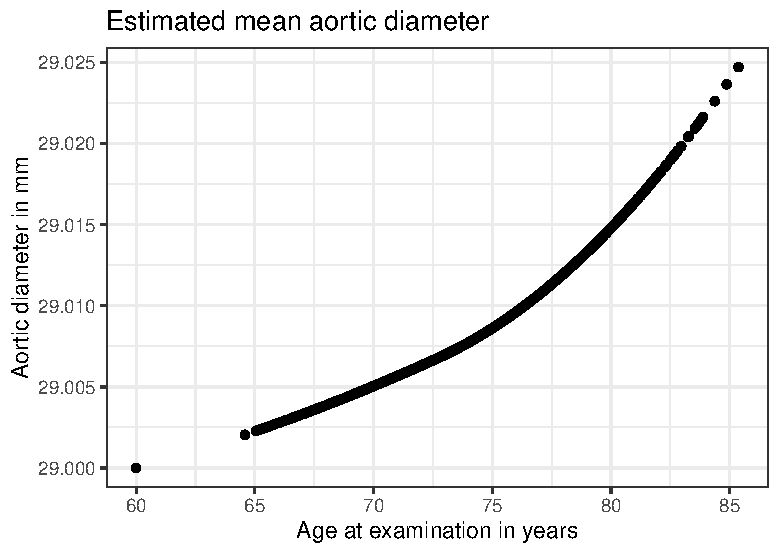
\includegraphics[scale=0.6]{Figures/fig_aneur_2diam_estimamean} &
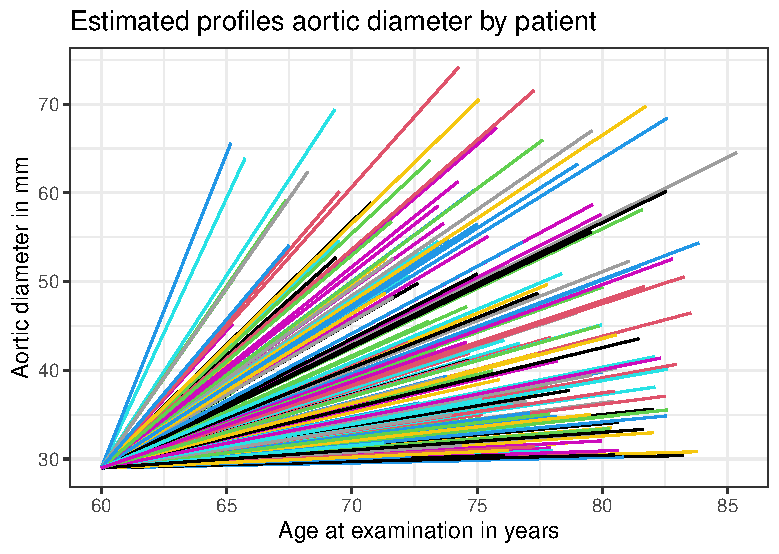
\includegraphics[scale=0.6]{Figures/fig_aneur_2diam_estimapos} 
\end{tabular}
%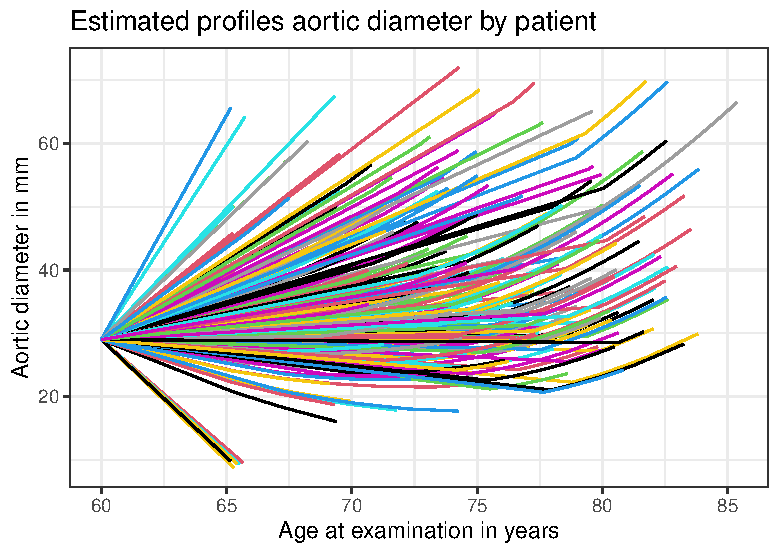
\includegraphics[scale=0.6]{Figures/fig_aneur_2diam_estima} 
\caption{Aortic aneurysm progression data: estimated profiles.}\label{fig:aneur.2estimate}
\end{figure}



Now, let $state_{it}$ be the ordinal response  variable of the stage of aneurysm for subject $i$ at time $t$. This ordinal response is modelled in terms of the cumulative probabilities $P(state_{it} \leq j | \boldsymbol{b}_i)$ by using the proportional odds model:  
 \begin{eqnarray*}
 P(state_{it} \leq j | \boldsymbol{b}_i) &=& \eta_{it,j}, 
 \end{eqnarray*}
with $j=1,2,3$,  subject to 
\begin{eqnarray*}
\eta_{it,j} &=& \kappa_{j} + f_1(age_{it}) +age_{it} \times b_{1i} , 
\qquad 
b_{1i}\sim\mathrm{N}(0,\psi^2), 
\end{eqnarray*}
where the constraints are such that $f_1$ is a non-decreasing smoothing function and $b_{1i}>0$, and for the breakpoints $\kappa_{j}<\kappa_{j+1}$. 


By using again 5 knots, Table \ref{tab:aneur.3estimate} presents a summary of the posterior estimates for the parameters of the ordinal model.  

\begin{table}[!htb] 
\centering 
\caption{Aortic aneurysm data: summary of the posterior estimates of the parameters. }\label{tab:aneur.3estimate}  
\begin{tabular}{cccccc} 
\hline 
\textbf{Parameter} & \textbf{Mean} & \textbf{Median} & \textbf{SD} & \textbf{2.5\%} & \textbf{97.5\%} \\ 
\hline 
$\gamma_1$ & 
1.04 & 1.02 & 0.17 & 0.73 & 1.45 \\ 
$\gamma_2$ & 
0.33 & 0.33 & 0.10 & 0.13 & 0.52 \\ 
$\gamma_3$ & 
1.36 & 1.36 & 0.21 & 0.97 & 1.78 \\ 
$\kappa_1$ & 
4.94 & 4.86 & 0.73 & 3.78 & 6.57 \\ 
$\kappa_2$ & 
11.70 & 11.60 & 0.87 & 10.27 & 13.64 \\ 
$\kappa_3$ & 
15.54 & 15.42  & 0.94 & 13.97 & 17.62 \\ 
$\psi^2$ & 
0.23 & 0.23 & 0.05 & 0.16 & 0.34 \\ 
$\log(\lambda)$ & 
5.98 & 5.98  & 0.41 & 5.16 & 6.77 \\ 
\hline 
\end{tabular} 
\end{table} 





\subsection{UPDRS scores data}


Let $y_{it}$ be the continuous response variable for the  Total UPDRS score, for subject $i$ at time $t$, $i=1,\ldots,n$, $t=1,\ldots,T_i$, and $n=42$, and  for the explanatory variables let $\boldsymbol{x}_{it}$ be the six acoustic features
JittP, 
LShimm, 
HNR, 
RPDE, 
DFA and
 PPE, related by the GAMM:  
\begin{eqnarray*}
y_{it} &=& f_1(x_{it1}) + \cdots + f_6(x_{it6})  + f_7(t) + b_{0i} + \varepsilon_{it}, 
\qquad 
b_{0i}\sim\mathrm{N}(0,\psi^2), 
\quad 
\varepsilon_{it}\sim\mathrm{N}(0,\sigma^2)  ,
\end{eqnarray*}
where $f_1,\ldots,f_6$ are non-constrained smoothing functions for the six acoustic features $x_{it1},\ldots,x_{it6}$, and $f_7$ is non-decreasing smoothing function; $b_{0i}$ is the random intercept; $\psi^2$ is the variance for the random intercept, and $\sigma^2$ is the common variance for the errors $\varepsilon_{it}$, having independent errors. 

The constraints used for the model allow to get results that seem to be in agreement with the dynamic progression of the disease. 

Figure \ref{fig:updrs.2estimate} displays the results. 

\begin{figure}[!htb]
\centering
\begin{tabular}{@{\hspace{0mm}}c@{\hspace{1mm}}c@{\hspace{1mm}}c@{\hspace{0mm}}}
%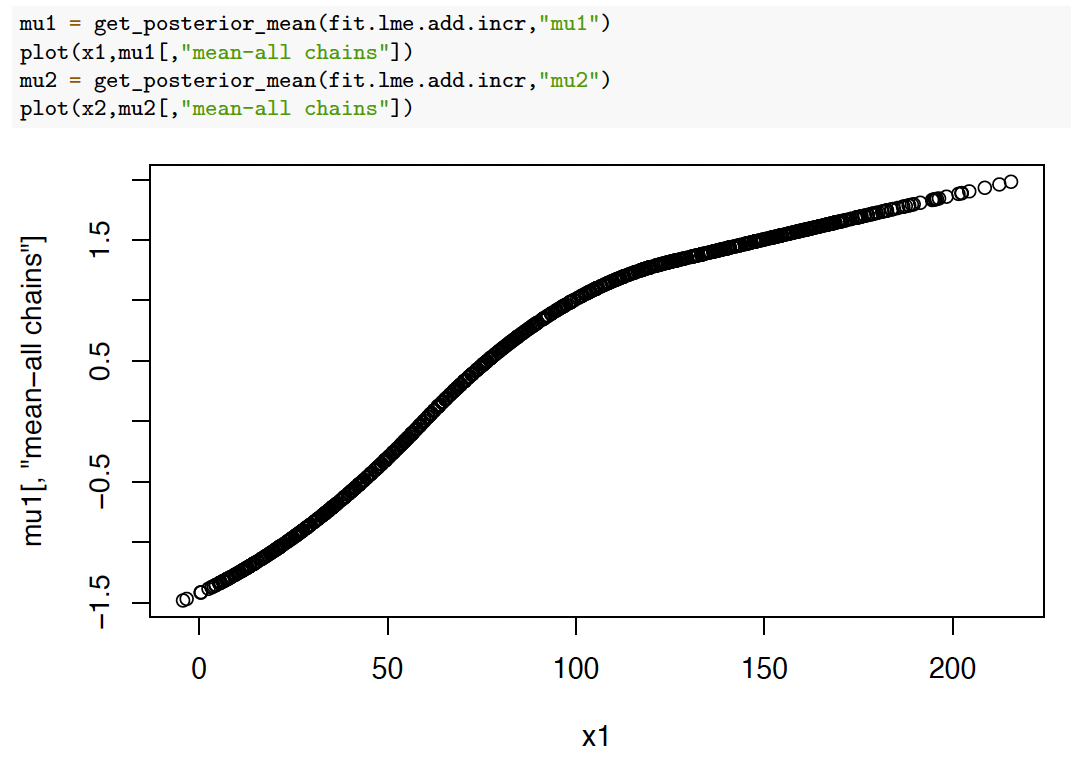
\includegraphics[scale=0.5]{Figures/fig_updrs_2estimate} &
%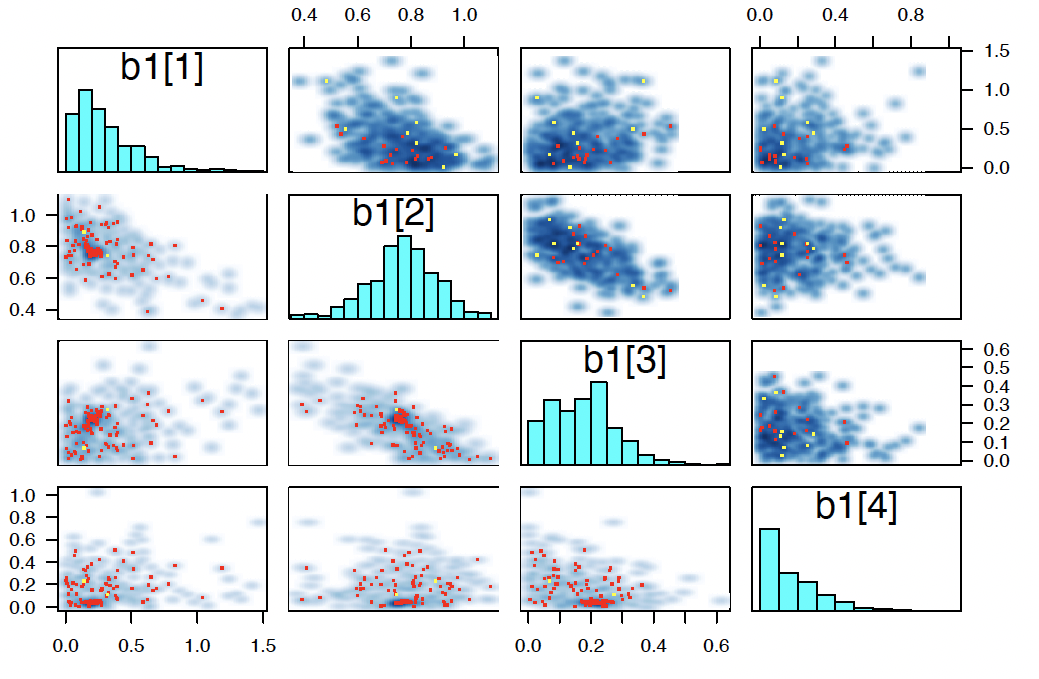
\includegraphics[scale=0.5]{Figures/fig_updrs_2posterior} 
\end{tabular}
\caption{UPDRS scores data: Results.}\label{fig:updrs.2estimate}
\end{figure}





\subsection{HIV: CD4-CD8 ratio and Adherence}


Let $y_{it}$ be the  CD4-CD8 ratio, the dependent variable,  for subject $i$ at time $t$, $i=1,\ldots,n$, $t=1,\ldots,T_i$, and $n=988$  patients. It is related to some features of patients:  
the ART adherence (ADH) measure in a continuous range of $0-100\%$,  
the time of the observation $t$,  
and the explanatory variables $\boldsymbol{x}_{it}$, corresponding to 
sex (male vs. female), 
age in years at ART initiation, 
and 
AIDS-related conditions indicator previous to enrollment in care (yes or no). 
For the GAMM logarithmic scale is used to improve the assumptions behind the model,  
\begin{eqnarray*} 
\log\left(y_{it}\right)  &=&  \boldsymbol{x}_{it}\boldsymbol{\beta}  +   f_1(ADH_{it}) + f_2(t) + b_{0i} + t\times b_{1i}  + \varepsilon_{it} , 
\qquad 
\boldsymbol{b}_i\sim\mathrm{N}(\boldsymbol{0},\boldsymbol{\psi}), 
\quad 
\boldsymbol{\varepsilon}_i\sim\mathrm{N}(\boldsymbol{0},\boldsymbol{\Lambda}\sigma^2)  ,
\end{eqnarray*}
where $f_1$ is a monotone smoothing function for the ART adherence $ADH_{it}$, $f_2$ is a non-constrained smoothing function for the time $t$; and for the random effects we consider $b_{0i}$ and $b_{1i}$ the random intercept and random slope, respectively, having normal distribution with mean $\boldsymbol{0}$ and covariance matrix $\boldsymbol{\psi}$; and the errores $\boldsymbol{\varepsilon}_{i}$ are independent normal distributed, having mean $\boldsymbol{0}$, non-correlated, common variance $\sigma^2$, and covariance matrix $\boldsymbol{\Lambda}$ for correlations.  



Figure \ref{fig:hiv.2estimate} displays the results. 

\begin{figure}[!htb]
\centering
\begin{tabular}{@{\hspace{0mm}}c@{\hspace{1mm}}c@{\hspace{1mm}}c@{\hspace{0mm}}}
%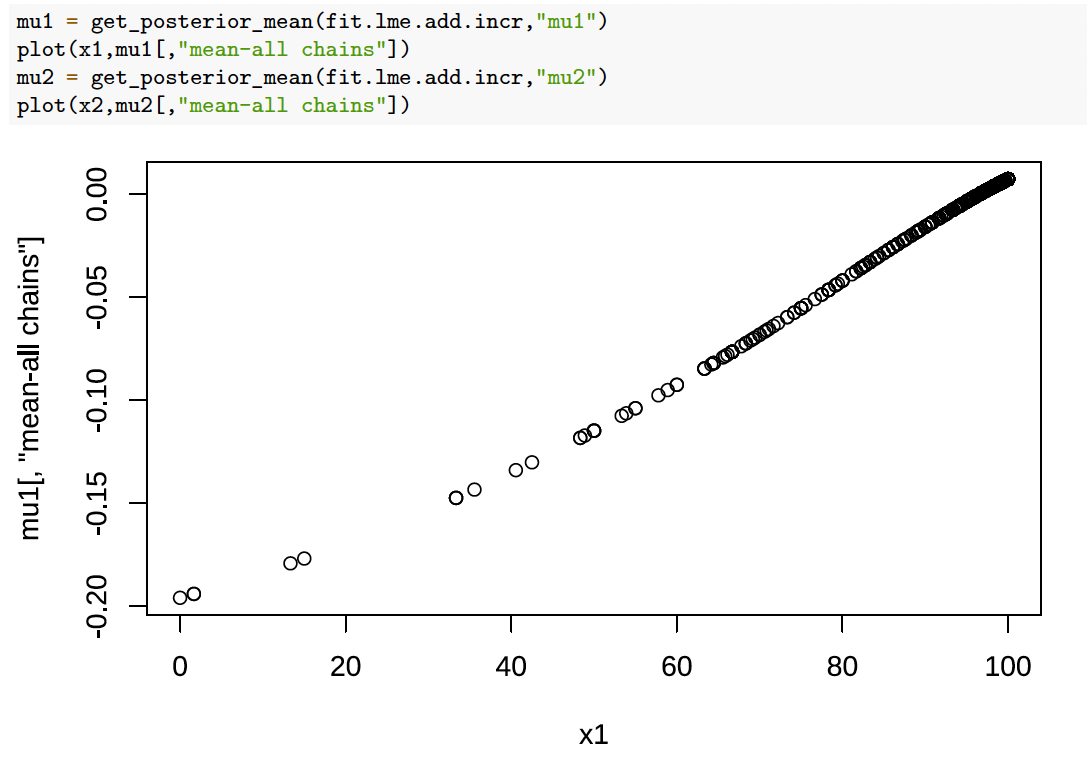
\includegraphics[scale=0.5]{Figures/fig_hiv2_estimate1} &
%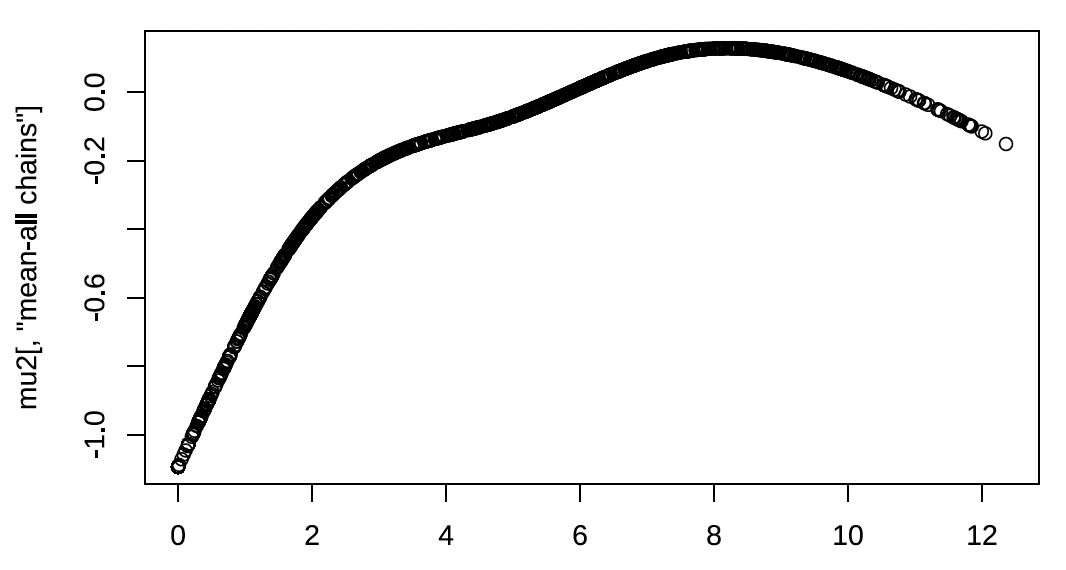
\includegraphics[scale=0.5]{Figures/fig_hiv2_estimate2} 
\end{tabular}
\caption{HIV: Results.}\label{fig:hiv.2estimate}
\end{figure}





%\clearpage 
\section{Conclusion}\label{sec:conclusion}

A Bayesian approach for generalized additive models has been proposed  to address  monotonicity constraints in the response. The proposed Bayesian models has been implemented by using STAN, and has been applied to track the monotony progression in some databases. 
With the examples used, we have shown that the proposal is applicable to different monotonicity processes whose response variable could be continuous,  ordinal, or  binary, subject to possible measurement errors or possible lack of information that leads to not fulfilling the natural monotonicity constraint. 


%\textbf{Parag. La ventaja de usar los GAMM frente a los GLMM} 

In statistical modeling strong parametric assumptions could lead to wrong conclusions.
As an alternative, nonparametric estimation methods have emerged, which make vague assumptions about the models and the data. 
For instances,  avoiding to make assumptions about the probability distribution that data follow,  and only relying on assumptions of independence; or instead of making assumptions of linearity for the relationship that may exist between variables, allows to non-linear patterns and use smoothing functions. 
So that GAM and GAMM as the nonparametric versions of GLM and GLMM, allow non-linear relationships including the smoothing functions, keeping the properties that GLM and GLMM have. 
 

%\textbf{Parag. Sobre las restricciones de monotonia}

Errors can be produced in the measuring processes or in the data collection processes. 
In some cases where data should follows a specific pattern, measurement errors may occur, and result in observed dada having different patterns to the ones are expected. For instance, when a disease has a degenerative nature,  being  characterized  by a progressive decline and have no cure, it is expected data follows non-increasing patterns through time, or non-decreasing, depending of the kind of biomarker  is used to monitor progression. 
When  measurement errors occur it is needed to include additional parameters or additional constraints in the statistical modeling to correct the bias in the parameters estimation and the predictions. 


%\textbf{Parag. sobre las ventajas de nuestra propuesta }\\ 

The proposed Bayesian approach fills in a gap on modelling longitudinal data by using generalized additive models with random effects  and having monotone constraints. 
By using the I-splines for the monotone constraints allows to implement the Bayesian approach in Stan in an easy way. 
Source codes for \texttt{R} and \texttt{Stan} for the examples presented in this paper are available through the GitHub repository \url{https://github.com/lizbethna/GAMBayes.git}. 


%\textbf{Qu\'e otros temas se pueden considerar:} \\ 

In the examples that motivated this work, we focused on longitudinal data for which their nature required compliance with the monotonicity constraint. 
However, as future works, some extensions can be considered for longitudinal data with constraints.
To consider other types of constraints on the smoothing functions,  as those studied by Mary C. Meyer \citep{Mey18,LiaMey19} of convexity, concavity and combinations of them to address longitudinal data.
To build up smooths of multiple variables, as the proposal studied by Pya and Wood \citep{PyaWoo15}, to model longitudinal data with constraints.
Our examples consider non-correlation structures on the observations of a  subject, however, more complex correlation structures can be considered, making some changes in the \texttt{Stan} codes.
Perhaps other two topics that have been less studied within additive models, that would represent a challenge in modeling longitudinal data, filling in two gaps, are models with multiple response like the vector generalized additive models (VGAM) \citep{Yee15},  and latent class models \cite{MutAsp09,ProPhiLiq17} to allow dividing a heterogeneous population into homogeneous subpopulations.


%\textbf{Parag. sobre la selecci\'on de los I-splines o los Integrated P-splines} \\ 
%*** Explicar las deferencias que existen entre los I-splines y los P-splines. \\



\section*{Acknowledgments}

This work was supported by UNAM PASPA-DGAPA, and by UNAM PAPIIT-DGAPA (Project IN100823), Mexico.

Victor Miranda **Acknowledgments**

Patricio Maturana **Acknowledgments**

\bibliographystyle{apalike}
\renewcommand\refname{Bibliograf\'ia}
\renewcommand\bibname{Bibliograf\'ia}
%\bibliographystyle{apalike-es}
\bibliography{bibliogeneral}



\end{document}